\chapter{邻接矩阵}

邻接矩阵用于描述点之间的连通关系,方便起见暂时只讨论简单无向图(无重边、无自环)邻接矩阵的性质,故下文中的图,若无特殊标明,均代表简单无向图。

%——————————————————————————————————%

\section{简单图}

先考虑较为一般的简单图。

\begin{definition}[简单图的邻接矩阵]
给定一个简单图 $\Gamma$,点集 $V\Gamma = {v_1, v_2, \dots, v_n}$,边集 $E\Gamma$ 是 $V\Gamma$ 中一些无序二元组构成集合,若 $\{v_i, v_j\} \in E\Gamma$,则称 $v_i$ 与 $v_j$ 是\textbf{邻接}(adjacent)的。

简单图 $\Gamma$ 的邻接矩阵是 $n\times n$ 的实对称矩阵 $\textbf A = \textbf A(\Gamma)$,其中元素定义为:
\[
a_{ij} = \begin{cases}
  1, \text{if $v_i$ and $v_j$ are adjacent;} \\ 
  0, \text{otherwise.}
\end{cases}
\]
\end{definition}

我们对定义出来的邻接矩阵的性质很感兴趣,不妨暂且研究其代数性质。因为没有自环,可以简单得到 $\text{tr}(\textbf A) = 0$。而图在任意重标号后仍然是不变的,所以在重标号后的矩阵也会有一些相似性,谱性质正是在行和列进行轮换过程中的不变量。

实对称矩阵具有很优美的性质:

\begin{theorem}[对称矩阵的谱定理]
一个对称的 $n\times n$ 矩阵 $\textbf A$ 具有下述性质:
\begin{enumerate} 
\item $\textbf A$ 有 $n$ 个特征值均为实数,包含重复的特征值,且每一个特征值的代数重数等于代数重数;

\item 特征空间相互正交,$\textbf A$ 可正交对角化。
\end{enumerate} 
\end{theorem}


\begin{proof}
先证明其特征值为实数。可以使用共轭来证明一个数是实数,即 $a\in \mathbb R \Leftrightarrow a = \bar a$。若 $\textbf A x = \lambda x$,注意到 $\textbf A\bar x = \bar{\textbf A}\bar x = \overline{\textbf Ax} = \overline{\lambda x} = \bar\lambda\bar x$,又有 $\textbf A^{T} = \textbf A$,于是考虑凑 $\textbf Ax$ 来得到 $\lambda$ 与 $\bar \lambda$:
\[
\overline {x^T}\textbf Ax\begin{cases}
= \overline {x^T\textbf A^T}x = \overline {(\textbf Ax)^T}x = \bar\lambda \overline {x^T}x
\\
= \overline {x^T}(\textbf Ax) = \overline {x^T}(\lambda x) = \lambda \overline {x^T}x
\end{cases}
\]

得到 $(\bar \lambda-\lambda)\overline {x^T}x = 0$,由 $\overline {x^T}x = \sum_{i = 1}^n x_i^2 \neq 0$,故 $\bar \lambda-\lambda = 0$,即 $\lambda$ 均为实数。

下面证明任意两特征向量正交:设 $\boldsymbol{v}_{1}$ 与 $\boldsymbol{v}_{2}$ 是不同特征值 $\lambda_1, \lambda_2$ 的特征向量,为证明 $v_1 \cdot v_2 = 0$,计算:
\[
\begin{aligned}
\lambda_{1} \boldsymbol{v}_{1} \cdot \boldsymbol{v}_{2} &=\left(\lambda_{1} \boldsymbol{v}_{1}\right)^{\mathrm{T}} \boldsymbol{v}_{2}=\left(A \boldsymbol{v}_{1}\right)^{\mathrm{T}} \cdot \boldsymbol{v}_{2} \\
&=\left(\boldsymbol{v}_{1}^{\mathrm{T}} A^{\mathrm{T}}\right) \boldsymbol{v}_{2}=\boldsymbol{v}_{1}^{\mathrm{T}}\left(A \boldsymbol{v}_{2}\right) \\
&=\boldsymbol{v}_{1}^{\mathrm{T}}\left(\lambda_{2} \boldsymbol{v}_{2}\right) \\
&=\lambda_{2} \boldsymbol{v}_{1}^{\mathrm{T}} \boldsymbol{v}_{2}=\lambda_{2} \boldsymbol{v}_{1} \cdot \boldsymbol{v}_{2}
\end{aligned}
\]

又 $\lambda_{1} \neq \lambda_{2}$,故有 $\boldsymbol{v}_{1} \cdot \boldsymbol{v}_{2} = 0$。

通过这两个性质可以得到剩下部分的证明,笔者能力有限,这里给不出证明。
\end{proof}

不妨通过邻接矩阵定义图的谱:

\begin{definition}[谱]
图 $\Gamma$ 的谱(spectrum)被定义为包含 $\textbf A(\Gamma)$ 的特征值及重数的集合。若有 $s$ 个不同的特征向量 $\lambda_0 > \lambda_1 > \dots > \lambda_{s-1}$,以及它们的重数 $m(\lambda_0) , m(\lambda_1) , \dots , m(\lambda_{s-1})$,我们可以将其写作:
\[
\text{Spec }\Gamma = 
\begin{pmatrix}
 \lambda_0 & \lambda_1 & \dots & \lambda_{s-1} \\
 m(\lambda_0) & m(\lambda_1) & \dots & m(\lambda_{s-1})
\end{pmatrix}
\]
\end{definition}

例如对于完全图 $K_4$ 的邻接矩阵:
\[
\textbf A = 
\begin{bmatrix}
 0 & 1 & 1 & 1\\
 1 & 0 & 1 & 1\\
 1 & 1 & 0 & 1\\
 1 & 1 & 1 & 0
\end{bmatrix}
\]
可以简单地求出它的谱为:
\[
\text{Spec } K_4=\begin{pmatrix}
 3 & -1 \\
 1 & 3
\end{pmatrix}
\]

为了找到这些代数量与图的关系,我们称 $\textbf A = \textbf A(\Gamma)$ 的特征值为图 $\Gamma$ 的特征值,特征多项式 $\det(\lambda \textbf I - \textbf A)$ 被称为图 $\Gamma$ 的特征多项式,并用 $\chi(\Gamma; \lambda)$ 表示,它通常是这样的形式:
\[
\chi(\Gamma ; \lambda)=\lambda^{n}+c_{1} \lambda^{n-1}+c_{2} \lambda^{n-2}+c_{3} \lambda^{n-3}+\ldots+c_{n}
\]

我们发现 $\chi(\Gamma; \lambda)$ 和图的形状有些关联。

\begin{proposition}[图的特征多项式的系数]
图 $\Gamma$ 的特征多项式 $\chi(\Gamma ; \lambda)=\lambda^{n}+c_{1} \lambda^{n-1}+c_{2} \lambda^{n-2}+c_{3} \lambda^{n-3}+\ldots+c_{n}$ 有如下性质:
\begin{enumerate} 
\item $c_1 = 0$;
\item $-c_2$ 是 $\Gamma$ 中边的条数;
\item $-c_3$ 是 $\Gamma$ 中三角形(三元环)的数量。
\end{enumerate} 
\end{proposition}

\begin{proof}
\begin{enumerate} 
\item $c_1 = 0$ 是显然的,因为 $\text{tr}(\textbf A) = 0$。
\item 考虑两行的主子式,若其非零,只能是形如
\[
\begin{bmatrix}
 0 & 1\\
 1 & 0
\end{bmatrix}
\]
的形式,且该主子式存在,当且仅当这两行对应的有连边。注意到该主子式的值为 $-1$,故 $(-1)^2 c_2 = -|E\Gamma|$,其中 $|E\Gamma|$ 是边集的大小。
\item 证明类似 2,我们取出三行的主子式:
\[
\left|\begin{array}{lll}
0 & 1 & 0 \\
1 & 0 & 0 \\
0 & 0 & 0
\end{array}\right|,\left|\begin{array}{lll}
0 & 1 & 1 \\
1 & 0 & 0 \\
1 & 0 & 0
\end{array}\right|,\left|\begin{array}{lll}
0 & 1 & 1 \\
1 & 0 & 1 \\
1 & 1 & 0
\end{array}\right|
\]

分别表示:

\begin{center}
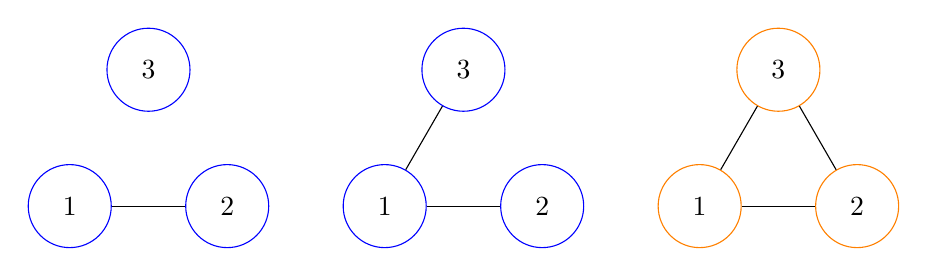
\begin{tikzpicture}
\node[circle,
minimum width =30pt ,
minimum height =30pt ,draw=blue] (1) at(0,0){1};
\node[circle,
minimum width =30pt ,
minimum height =30pt ,draw=blue] (2) at(2,0){2};
\node[circle,
minimum width =30pt ,
minimum height =30pt ,draw=blue] (3) at(1,1.732){3};
\node[circle,
minimum width =30pt ,
minimum height =30pt ,draw=blue] (4) at(4,0){1};
\node[circle,
minimum width =30pt ,
minimum height =30pt ,draw=blue] (5) at(6,0){2};
\node[circle,
minimum width =30pt ,
minimum height =30pt ,draw=blue] (6) at(5,1.732){3};
\node[circle,
minimum width =30pt ,
minimum height =30pt ,draw=orange] (7) at(8,0){1};
\node[circle,
minimum width =30pt ,
minimum height =30pt ,draw=orange] (8) at(10,0){2};
\node[circle,
minimum width =30pt ,
minimum height =30pt ,draw=orange] (9) at(9,1.732){3};
\draw[-] (1) --(2);

\draw[-] (4) --(5);
\draw[-] (4) --(6);

\draw[-] (7) --(8);
\draw[-] (7) --(9);
\draw[-] (8) --(9);
\end{tikzpicture}
\end{center}

不难发现只有第三种三元环对 $c_3$ 有贡献,且值为 $2$,这就得到了该性质。
\end{enumerate} 
\end{proof}

\begin{corollary}[特征多项式的约化公式]
对于图 $\Gamma$,若 $v_1$ 的度数为 $1$,且与 $v_2$ 相连,则有:
\[
\chi(\Gamma ; \lambda) = \lambda \chi(\Gamma_1 ; \lambda) - \chi(\Gamma_{12} ; \lambda)
\]

其中 $\Gamma_1$ 是删掉 $v_1$ 的导出子图,$\Gamma_{12}$ 是删掉 ${v_1, v_2}$ 的导出子图。
\end{corollary}
\begin{proof}
由于 $v_1$ 有大量的 $0$,故考虑用代数余子式进行展开。
\[
\left|
\begin{array}{c:ccc}
 \lambda & -1 & 0 & 0\\
 -1 & \lambda & \cdots & a_{2n}\\
 0 & \vdots & \ddots & \vdots\\
 0 & a_{n2} & \cdots & \lambda
\end{array}
\right|
=
\lambda \chi(\Gamma_1 ; \lambda)
-
\left|
\begin{array}{cccc} 
-1 & 0 & 0 & 0\\
\hdashline 
a_{32} & \lambda & \cdots & a_{3n} \\
\vdots & \vdots & \ddots & \vdots \\
a_{n2} & a_{n3} & \cdots & \lambda \\
\end{array}
\right|
=
\lambda \chi(\Gamma_1 ; \lambda) - \chi(\Gamma_{12} ; \lambda)
\]
\end{proof}

上面的公式可以用于快捷地求无环图的特征多项式,因为无论如何删除,必存在一个度为 $1$ 的点。

\begin{proposition}[特征值幂和]
令 $\textbf A = \textbf A(\Gamma)$,其特征根为 $\lambda_1, \lambda_2, \dots, \lambda_r$,则有:
\begin{enumerate} 
\item $\sum_{i = 1}^{r} \lambda_i^{2}$ 是 $\Gamma$ 中边数的 $2$ 倍;
\item $\sum_{i = 1}^{r} \lambda_i^{3}$ 是 $\Gamma$ 中三元环数量的 $6$ 倍。
\end{enumerate} 
\end{proposition}

\begin{proof}
这里只给出证明思路。
\begin{center}
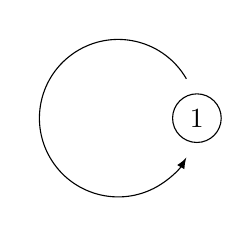
\begin{tikzpicture}

\def \n {1}
\def \radius {1cm}
\def \margin {30} % margin in angles, depends on the radius

\foreach \s in {1,...,\n}
{
  \node[draw, circle] at ({360/\n * (\s - 1)}:\radius) {$\s$};
  \draw[->, >=latex] ({360/\n * (\s - 1)+\margin}:\radius) 
    arc ({360/\n * (\s - 1)+\margin}:{360/\n * (\s)-\margin}:\radius);
}
\end{tikzpicture}
\quad
\begin{tikzpicture}

\def \n {2}
\def \radius {2cm}
\def \iradius {1.7cm}
\def \margin {14} % margin in angles, depends on the radius

\foreach \s in {1,...,\n}
{
  \node[draw, circle] at ({360/\n * (\s - 1)}:\radius) {$\s$};
  \draw[->, >=latex] ({360/\n * (\s - 1) + \margin}:\radius) 
    arc ({360/\n * (\s - 1)+\margin} : {360/\n * \s-(\margin * 10)}:\radius);
  \draw ({360/\n * \s}: \iradius) -- ({360/\n * (\s - 1)}: \iradius);
}
\end{tikzpicture}
\quad
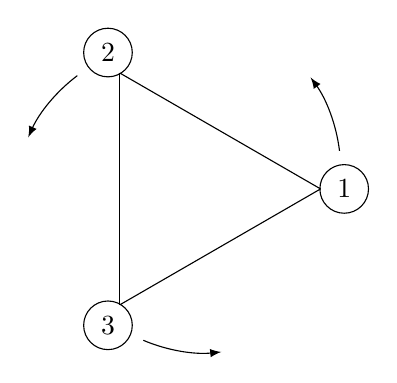
\begin{tikzpicture}

\def \n {3}
\def \radius {2cm}
\def \iradius {1.7cm}
\def \margin {7} % margin in angles, depends on the radius

\foreach \s in {1,...,\n}
{
  \node[draw, circle] at ({360/\n * (\s - 1)}:\radius) {$\s$};
  \draw[->, >=latex] ({360/\n * (\s - 1) + \margin * 2}:\radius) 
    arc ({360/\n * (\s - 1)+\margin}:{360/\n * (\s)-(\margin * 12)}:\radius);
  \draw ({360/\n * \s}: \iradius) -- ({360/\n * (\s - 1)}: \iradius);
}
\end{tikzpicture}
\end{center}
注意在图上的回路,例如长度为 $l$ 的回路的条数等于 $\text{tr }\textbf A^l$。
\end{proof}

在这个命题中,给出了它们各种幂次和的值,从 $\sum \lambda_i = 0, \sum \lambda_i^2 = 2m$ 可见 $\lambda$ 存在一个上界。

\begin{proposition}[特征值上界]
若 $\lambda_0 = \max_{i}\{\lambda_i\}$,则有
\[
\lambda_0 \le \left(\frac{2m(n - 1)}{n}\right)^{\frac 1 2}
\]
另一种类似形式的上界是 $\lambda_0 \le \sqrt{2m - n + 1}$(Yuan 1988)。
\end{proposition}
\begin{proof}
不会,但是感觉能做,先放着等回来填坑。
\end{proof}

关于特征多项式的更多性质要等到后面才学,不写了。

\begin{definition}[邻接代数]
定义在图 $\Gamma$ 上的邻接代数(adjacency algebra)是邻接矩阵 $\textbf A = \textbf A(\Gamma)$ 的多项式形式的代数,记作 $\mathcal A(\Gamma)$,其每一个元素都是 $\textbf A$ 的幂的线性组合。
\end{definition}

$\textbf A$ 的幂有什么性质,为什么这样定义代数呢?

首先对于图 $\Gamma$ 中起点为 $v_i$,终点为 $v_j$,且长度为 $l$ 的一条路径(walk),我们将其写为数列的形式:$\{u_0, u_1, u_2, \dots, u_l\}$,其中 $u_0 = v_i, u_l = v_j$,其中 $u_{t - 1}, u_t, t\in{1,2,\dots,l}$ 是连通的。

\begin{theorem}
图 $\Gamma$ 中起点为 $v_i$,终点为 $v_j$,且长度为 $l$ 的路径的条数为 $\textbf A^l$ 中 $(i, j)$ 位置的值。
\end{theorem}

\begin{proof}
考虑归纳法:
\begin{enumerate}
\item $l = 1$ 时显然成立;
\item 若 $l = L$ 成立,下面证明 $l = L + 1$ 时成立:

考虑与 $v_j$ 相邻的节点 $v_h$,则起点为 $v_i$,终点为 $v_j$,且长度为 $L + 1$ 的路径必经过 $v_h$,且到 $v_h$ 的长度为 $L$,所以统计 $v_i$ 到 $v_h$ 的路径条数:
\[
\sum_{\left\{v_{h}, v_{j}\right\} \in E \Gamma}\left(\mathbf{A}^{L}\right)_{i h}
=\sum_{h=1}^{n}\left(\mathbf{A}^{L}\right)_{i h} a_{h j}
=\left(\mathbf{A}^{L+1}\right)_{i j}
\]
满足题中形式,故成立。
\end{enumerate}

综上,对于 $l \in \mathbb N^*$,该性质成立。
\end{proof}

如果 $\Gamma$ 中任意两个顶点存在一条路径经过他们,则称 $\Gamma$ 是连通(connected)的。连接 $v_i, v_j$ 的路径中最短的长度称为 $v_i, v_j$ 的距离(distance),记作 $\partial (v_i, v_j)$。图 $\Gamma$ 的直径(diameter)定义为 $\sup_{x,y\in V\Gamma} \partial (x, y)$。

\begin{theorem}
连通图 $\Gamma$ 中的邻接代数 $\mathcal A(\Gamma)$ 与直径 $d = \sup_{x,y\in V\Gamma} \partial (x, y)$ 满足:
\[
d + 1 \le \dim \mathcal A(\Gamma)
\]
\end{theorem}
\begin{proof}
取 $\partial (x, y) = d$,即存在一条路径 $\{w_0, w_1, \dots, w_d\}, w_0 = x, w_d = y$,不难发现,对于 $w_n, w_m$,有 $\partial(w_n, w_m) = |n - m|$。故 $\forall l \in {1, 2, \dots, d}, \exists p,q\in [0,d], \partial(p, q) = l$,由上一个定理不难得到,存在一个位置 (p, q),有 $(\textbf A^i)_{pq} \neq 0$,且 $\textbf I, \textbf A, \textbf A^2, \dots, \textbf A^{i - 1}$ 在这个位置为 $0$。所以 $\{\textbf I, \textbf A, \textbf A^2, \dots, \textbf A^d\}$ 线性无关,共有 $d + 1$ 个元素,得到 $d + 1 \le \dim \mathcal A(\Gamma)$。
\end{proof}

图的谱和邻接代数有密切的联系。邻接矩阵作为实对称矩阵,其最小多项式次数与邻接代数的维度相等,所以我们找到了不同特征根的数量的上界:

\begin{corollary}
直径为 $d$ 的连通图至少有 $d + 1$ 个特征根。
\end{corollary}

下面来看一个例子:

\begin{proposition}[完全图的谱]
\[
\operatorname{Spec}\left(K_{n}\right)=\left(\begin{array}{cc}
-1 & n-1 \\
n-1 & 1
\end{array}\right)
\]
\end{proposition}

\begin{proof}
直接计算:
\[
\begin{aligned}
\left|\lambda \textbf I-\textbf{A} \left(K_{n}\right)\right|
&=
\left|\begin{array}{cccc}
\lambda & -1 & \cdots & -1 \\
-1 & \lambda & \cdots & -1 \\
\vdots & \vdots & \ddots & \vdots \\
-1 & -1 & \cdots & \lambda
\end{array}\right|
=
\left|\begin{array}{cccc}
\lambda - n + 1 & -1 & \cdots & -1 \\
\lambda - n + 1 & \lambda & \cdots & -1 \\
\vdots & \vdots & \ddots & \vdots \\
\lambda - n + 1 & -1 & \cdots & \lambda
\end{array}\right|\\
&=
(\lambda - n + 1)\left|\begin{array}{cccc}
1 & -1 & \cdots & -1 \\
1 & \lambda & \cdots & -1 \\
\vdots & \vdots & \ddots & \vdots \\
1 & -1 & \cdots & \lambda
\end{array}\right|
=(\lambda - n + 1)(\lambda + 1) ^ {n - 1}
\end{aligned}
\]
故
\[
\operatorname{Spec}\left(K_{n}\right)=\left(\begin{array}{cc}
-1 & n-1 \\
n-1 & 1
\end{array}\right)
\]
\end{proof}



%——————————————————————————————————%

\section{正则图}

下面研究特殊图的性质。

\begin{definition}[正则图]
一个图被称为正则(regular)或$k$-正则($k$-regular)的,当且仅当每个顶点的度数为 $k$。
\end{definition}

正则图的邻接矩阵每行每列的和是相同的,所以会有一些有意思的性质。

\begin{theorem}[正则图特征值的性质]
若 $\Gamma$ 是一个 $k$-正则图,则有:
\begin{enumerate}
\item $k$ 是 $\Gamma$ 的一个特征值;
\item 如果 $\Gamma$ 连通,则 $k$ 的重数为 $1$;
\item 特征值绝对值的上界为 $k$。
\end{enumerate}
\end{theorem}
\begin{proof}
\begin{enumerate}
\item 注意到对于$k$-正则图的邻接矩阵,每行每列的和都为 $k$,可构造 $\textbf u = [1,1,\dots,1]^T$,有 $\textbf{Au} = k\textbf u$,故 $k$ 是 $\Gamma$ 的一个特征值;
\item 注意 $\textbf x$ 左乘 $\textbf A$ 相当于对于每个位置,选取 $k$ 个与其相邻的数相加,所以关注 $\textbf x$ 中的最大值,记为 $x_j$。有 $(\textbf{Ax})_j = k x_j \Leftrightarrow \sum_{i}x_i = k x_j$,其中 $i$ 代表与 $j$ 邻接的点。这个式子中,由 $x_i \le x_j$,得到 $x_i = x_j$,再对 $i$ 进行操作,可将这个性质传递到整个连通块,也就是整个图。故 $\textbf x = x_j \textbf u$,也就是所有的 $\textbf x$ 都是 $\textbf u$ 的倍数,$x$ 的重数为 $1$。
\item 过程与 $2$ 相似,不过取绝对值最大的元素 $y_j$,可以得到 $|\lambda||y_j| = |\sum_i y_i| \le \sum_i|y_i| \le k|y_j|$,故 $|\lambda| \le k$。
\end{enumerate}
\end{proof}

\begin{proposition}[Hoffman 1963]
令 $\textbf J$ 是 $n\times n$ 的全 $+1$ 矩阵,则 $\textbf J \in \mathcal A(\Gamma)$ 当且仅当 $\Gamma$ 连通且正则。
\end{proposition}
\begin{proof}
\begin{enumerate}
\item 先证 “$\Rightarrow$”:
\begin{enumerate}
\item 由 $\textbf J \in \mathcal A(\Gamma)$,故 $\textbf J$ 可以被表示为关于 $\textbf A$ 的多项式。因为 $\textbf A$ 与 $\textbf J$ 都是实对称矩阵,故 $\textbf {JA} = \textbf {AJ}$,考虑位置 $(i,j)$,由 $\sum_{k = 1}^n \textbf A_{kj} = \sum_{k = 1}^n \textbf A_{ik}$,即点 $i$ 的度数与点 $j$ 的度数相等,故 $\Gamma$ 是正则图;
\item 若 $\Gamma$ 不连通,即存在点对 ${v_i, v_j}$ 之间没有路径连通,则 $\forall l > 0, \textbf A^l_{ij} = 0$,而 $\textbf J_{ij} \neq 0$,矛盾!;
\end{enumerate}
\item 再证 “$\Leftarrow$”:

令 $\Gamma$ 为连通且$k$-正则的,则 $k$ 是 $\Gamma$ 的一个特征值,所以 $\textbf A$ 的最小多项式 $p(\lambda)$ 满足 $p(\lambda) = (\lambda - k) q(\lambda)$ 的形式,由 $p(\textbf A)$,带入得 $\textbf A q(\textbf A) = kq(\textbf A)$,这意味着 $q(\textbf A)$ 的每一列都是 $\textbf A$ 关于特征值 $k$ 的特征向量,由定理1.4,$q(\textbf A)$ 的每一列都是 $\textbf u$ 的倍数。又 $q(\textbf A)$ 是对称矩阵,得到 $q(\textbf A)$ 的元素全部相等,是 $\textbf J$ 的倍数,故 $\textbf J \in \mathcal A(\Gamma)$。
\end{enumerate}
\end{proof}

我们还可以进一步得到 $q(\textbf A)$ 与 $\textbf J$ 的关系:

\begin{proposition}
令 $\Gamma$ 是一个 $n$ 个点$k$-正则的连通图,将它们不同的特征值记为 $k > \lambda_1 > \dots > \lambda_{s - 1}$,若 $q(\lambda) = \prod_i (\lambda - \lambda_i)$,有:
\[
\textbf J = \left(\frac {n} {q(k)}\right) q(\textbf A)
\]
\end{proposition}

\begin{proof}
由上一个命题知 $q(\textbf A) = \alpha \textbf J$,其中 $\alpha$ 是常数,下面考虑特征值。$\alpha \textbf J$ 的特征值是 $\alpha n$,而 $q(\textbf A)$ 有 $q(k)$ 与 $q(\lambda_i)$,但由题知仅有 $q(k) \neq 0$,故得到 $\alpha = q(k) / n$。
\end{proof}

这一部分与矩阵联系较为紧密,有许多重要的种类,不妨再来回顾一下相关的知识。

\begin{definition}[循环矩阵]
一个 $n\times n$ 的矩阵 $\textbf S$ 被成为循环矩阵(circulant matrix),当且仅当其中的元素满足 $s_{ij} = s_{1,j-i+1}$,$j-i+1$ 的计算是在模 $n$ 意义下的,故 $\textbf S$ 可以被看作是由第一行生成的,记作 $[s_1, s_2, \dots, s_n]$。

若令 $\textbf W$ 是单位循环矩阵,即 $\textbf W = [0,1,0,\dots,0]$,$S$ 可被表示为:

\[
\textbf S = \sum_{i = 1}^n s_i \textbf W^{i - 1}
\]
\end{definition}

可以注意到 $\textbf W$ 可以作为乘法循环群的生成元,可见特征值在该过程中有特殊的性质,我们有:

\begin{proposition}
$n$ 阶单位循环矩阵 $\textbf W$ 的特征值为 $1, \omega, \omega^2, \dots, \omega^{n - 1}$,其中 $\omega = \exp(2\pi i / n)$。由此得到 $\textbf S$ 的特征值为:
\[
\lambda_r = \sum_{i = 1}^n s_i \omega^{(i - 1)r}, r\in\{0, 1, \dots, n - 1\}
\]
\end{proposition}
\begin{proof}
直接计算:
\[
\begin{aligned}
|\lambda\textbf I - \textbf W| & = \left|
\begin{array}{c:ccc}
  \lambda & -1 & \cdots & 0 \\  
  0 & \lambda & \cdots & 0 \\  
  \vdots & \vdots & \ddots & \vdots \\  
  -1 & 0 & \cdots & \lambda  
\end{array}
\right| = \lambda \left|
\begin{array}{cccc}
  \lambda & -1 & \cdots & 0 \\  
  0 & \lambda & \cdots & 0 \\  
  \vdots & \vdots & \ddots & \vdots \\  
  0 & 0 & \cdots & \lambda  
\end{array}
\right|
+
(-1)^{n-1}\times (-1)\left|
\begin{array}{cccc}
  -1 & 0 & \cdots & 0 \\  
  \lambda & -1 & \cdots & 0 \\  
  \vdots & \vdots & \ddots & \vdots \\  
  0 & 0 & \cdots & -1 
\end{array}
\right|
\\
& = \lambda^n + (-1)^{2n-1}=\lambda^n - 1 = 0
\end{aligned}
\]
故可将 $\lambda$ 写成 $n$ 次单位根的形式。
\end{proof}

我们把循环矩阵的定义放到图中:

\begin{definition}[循环图]
图 $\Gamma$ 被称为循环图(circulant graph),当且仅当邻接矩阵 $\textbf A(\Gamma)$ 是循环矩阵。
\end{definition}

循环图 $\Gamma$ 的 $\textbf A$ 的第一行为 $[0, a_2, \dots, a_n]$,代入上面命题可得到:

\begin{theorem}[循环图的特征值]
循环图 $\Gamma$ 的特征值为:
\[
\lambda_r = \sum_{i = 2}^n a_i \omega^{(i - 1)r}, r\in\{0, 1, \dots, n - 1\}
\]
\end{theorem}

此时 $n$ 个特征值并非总是不同的。

对于一个 $n$ 元环构成的图,记为 $C_n$,$\textbf A(C_n)$ 的第一行为 $[0, 1, 0, \dots, 0, 1]$,由上面的定理可以得到其特征值为 $\lambda_r = 2\cos(2\pi r / n)$,可以得到 $C_n$ 的谱:

\[
\begin{aligned}
 \operatorname{Spec} C_{n} & = \left(\begin{array}{cccc}2 & 2 \cos 2 \pi / n & \ldots & 2 \cos (n-1) \pi / n \\ 1 & 2 & \ldots & 2\end{array}\right) \quad(n\text{ odd}) \\
 \operatorname{Spec} C_{n} & = \left(\begin{array}{ccccc}2 & 2 \cos 2 \pi / n & \ldots & 2 \cos (n-2) \pi / n & -2 \\ 1 & 2 & \ldots & 2 & 1\end{array}\right) \quad(n\text{ even}) 
\end{aligned}
\]

我们来看另一个可能暗示结构上的性质的图:

\begin{definition}[线图]
定义在 $\Gamma$ 上的线图(line graph)记为 $L(\Gamma)$,其每个顶点对应 $\Gamma$ 中的一条边,两个顶点是邻接的当且仅当它们代表的边有公共顶点。
\end{definition}

对于 $n$ 个顶点和 $m$ 条边的图,将其顶点与边标号可得 $V\Gamma = \{v_1, v_2, \dots, v_n\}$ 与 $E\Gamma = \{e_1, e_2, \dots, e_m\}$。我们定义图 $\Gamma$ 的关系矩阵 $\textbf X=\textbf X(\Gamma) \in \mathbb R^{n\times m}$:
\[
(\mathbf{X})_{i j}=\left\{\begin{array}{ll}
1, & \text { if } v_{i} \text { and } e_{j} \text { are incident } \\
0, & \text { otherwise }
\end{array}\right.
\]

可以得到关于 $\textbf X$ 的一些性质:

\begin{lemma}
对于图 $\Gamma$ 与如上定义的 $\textbf X$,令 $\textbf A = \textbf A(\Gamma), \textbf A_L = \textbf A(L(\Gamma))$,有:
\begin{enumerate}
\item $\textbf X^T\textbf X = \textbf A_L + 2\textbf I_m$
\item 若 $\Gamma$ 是 $k$-正则的,则 $\textbf X\textbf X^T = \textbf A_L + k\textbf I_n$
\end{enumerate}
\end{lemma}
\begin{proof}
写出矩阵乘的形式:
\[
(\textbf X^T\textbf X)_{ij} = \sum_{k = 1}^n (\textbf X)_{ki} (\textbf X)_{kj}
\]
注意到右侧正是 $\textbf A_L$ 的定义,第二条的证明与第一条相似。
\end{proof}

\begin{lemma}[线图特征值的下界]
对于 $L(\Gamma)$ 的任一特征值 $\lambda$,有 $\lambda \ge -2$。
\end{lemma}
\begin{proof}
矩阵 $\textbf X^T\textbf X$ 元素都是非负的,若 $\textbf X^T \textbf X \textbf z = \lambda \textbf z$,左乘 $\textbf z^T$,由 $\textbf z^T \textbf X^T \textbf X \textbf z = ||\textbf {Xz}||^2 \ge 0$,故 $\textbf X^T \textbf X$ 的特征值 $\lambda$ 非负,也就是 $|\lambda \textbf I - \textbf X^T\textbf X|=0$ 的解非负,由 $\textbf X^T\textbf X - 2\textbf I_m = \textbf A_L$ 可得 $A_L$ 的特征值不小于 $-2$。
\end{proof}

事实上,并非只有线图满足这个性质,更多满足该性质的图后面会补充。

正则图的线图仍然是正则图,对于$k$-正则图 $\Gamma$,线图 $L\Gamma$ 是$2(k-1)$-正则图,由正则图特征值的性质,正则图与其线图可能存在一些联系:

\begin{theorem}[Sachs 1967]
若 $\Gamma$ 是$k$-正则图,有 $n$ 个点与 $m = nk/2$ 条边,则有:
\[
\chi(L(\Gamma); \lambda) = (\lambda + 2)^{m - n} \chi (\Gamma; \lambda + 2 - k)
\]
\end{theorem}
\begin{proof}
构造两个 $n + m$ 阶的矩阵:
\[
\mathbf{U}=\left[\begin{array}{cc}
\lambda \mathbf{I}_{n} & -\mathbf{X} \\
\mathbf{0} & \mathbf{I}_{m}
\end{array}\right], \quad \mathbf{V}=\left[\begin{array}{cc}
\mathbf{I}_{n} & \mathbf{X} \\
\mathbf{X}^{T} & \lambda \mathbf{I}_{m}
\end{array}\right]
\]
可以得到它们的乘积:
\[
\mathbf{U V}=\left[\begin{array}{cc}
\lambda \mathbf{I}_{n}-\mathbf{X} \mathbf{X}^{T} & \mathbf{0} \\
\mathbf{X}^{T} & \lambda \mathbf{I}_{m}
\end{array}\right], \quad \mathbf{V U}=\left[\begin{array}{cc}
\lambda \mathbf{I}_{n} & \mathbf{0} \\
\lambda \mathbf{X}^{T} & \lambda \mathbf{I}_{m}-\mathbf{X}^{T} \mathbf{X}
\end{array}\right]
\]
由 $\det(\mathbf{U V}) = \det(\mathbf{V U})$,以及分块矩阵行列式的性质,可得 $\lambda^{m} \operatorname{det}\left(\lambda \mathbf{I}_{n}-\mathbf{X} \mathbf{X}^{T}\right)=\lambda^{n} \operatorname{det}\left(\lambda \mathbf{I}_{m}-\mathbf{X}^{T} \mathbf{X}\right)$,有:
\[
\begin{aligned}
\chi(L(\Gamma) ; \lambda) &=\operatorname{det}\left(\lambda \mathbf{I}_{m}-\mathbf{A}_{L}\right) \\
&=\operatorname{det}\left((\lambda+2) \mathbf{I}_{m}-\mathbf{X}^{T} \mathbf{X}\right) \\
&=(\lambda+2)^{m-n} \operatorname{det}\left((\lambda+2) \mathbf{I}_{n}-\mathbf{X} \mathbf{X}^{T}\right) \\
&=(\lambda+2)^{m-n} \operatorname{det}\left((\lambda+2-k) \mathbf{I}_{n}-\mathbf{A}\right) \\
&=(\lambda+2)^{m-n} \chi(\Gamma ; \lambda+2-k)
\end{aligned}
\]
\end{proof}

由 $\Gamma$ 的谱:
\[
\operatorname{Spec} \Gamma=\left(\begin{array}{cccc}
k & \lambda_{1} & \ldots & \lambda_{s-1} \\
1 & m_{1} & \ldots & m_{s-1}
\end{array}\right)
\]
可以得到 $L(\Gamma)$ 的谱:
\[
\operatorname{Spec} L(\Gamma)=\left(\begin{array}{ccccc}
2 k-2 & k-2+\lambda_{1} & \ldots & k-2+\lambda_{s-1} & -2 \\
1 & m_{1} & \ldots & m_{s-1} & m-n
\end{array}\right)
\]

\begin{proposition}
对于 $n$ 个点$k$-正则的连通图 $\Gamma$,定义其补图 $\Gamma^c$ 为有相同的点集,边集互补的图,也就是 $\mathbf A + \mathbf A_c = \mathbf J - \mathbf I$,则有:
\[
(\lambda + k + 1) \chi (\Gamma^c; \lambda) = (-1)^n (\lambda - n + k + 1) \chi (\Gamma; -\lambda - 1)
\]
\end{proposition}

\begin{proposition}
对于 $n$ 个点$k$-正则的连通图 $\Gamma$,定义其补图 $\Gamma^c$ 为有相同的点集,边集互补的图,也就是 $\mathbf A + \mathbf A_c = \mathbf J - \mathbf I$,则有:
\[
(\lambda + k + 1) \chi (\Gamma^c; \lambda) = (-1)^n (\lambda - n + k + 1) \chi (\Gamma; -\lambda - 1)
\]
\end{proposition}

% ========================================== %

\section{圈和割}

\begin{definition}[点空间与边空间]
图 $\Gamma$ 的点空间(vertex-space)记为 $C_0(\Gamma)$,代表所有映射 $f: V\Gamma \to \mathbb C$。
图 $\Gamma$ 的边空间(edge-space)记为 $C_1(\Gamma)$,代表所有映射 $f: E\Gamma \to \mathbb C$。
\end{definition}

令 $V\Gamma = \{v_1, v_2, \dots, v_n\}$,$E\Gamma = \{e_1, e_2, \dots, e_m\}$,知 $C_0(\Gamma),C_1(\Gamma)$ 分别是 $n,m$ 维的向量空间。又所有 $\eta: V\Gamma \to \mathbb C$ 可以被表示为一个列向量 $\textbf y = [y_1, y_2, \dots, y_n]^T$,其中 $y_i = \eta(v_i), i\in {1,2,\dots,n}$,于是我们可以定义一组基 $\{\omega_1, \omega_2, \dots, \omega_n\}$:
\[
\omega_i(v_j) = \left\{\begin{aligned} 
&1, &\text{ if } i=j \\  
&0, &\text{ otherwise}
\end{aligned}\right.
\]
以相同的方式也可以定义对于 $C_1(\Gamma)$ 的一组基 $\{\epsilon _1, \epsilon_2, \dots, \epsilon_m\}$:
\[
\epsilon_i(e_j) = \left\{\begin{aligned} 
&1, &\text{ if } i=j \\  
&0, &\text{ otherwise}
\end{aligned}\right.
\]

上面讨论的都是无向图,现在讨论边的定向:

\begin{definition}[关联矩阵]
$\Gamma$ 的关联矩阵(incidence matrix)记为 $\textbf D$,代表给 $\Gamma$ 定向,是一个 $n\times m$ 的矩阵,元素为:
\[
d_{ij} = \left\{\begin{aligned} 
&+1, &\; \text{ if } v_i \text{ is the positive end of } e_j; \\  
&-1, &\; \text{ if } v_i \text{ is the negatice end of } e_j; \\  
&0 , &\; \text{ otherwise.}
\end{aligned}\right.
\]
\end{definition}

$\textbf D$ 的每一列只有两个非零元素,可以将 $\textbf D$ 看作 $C_1(\Gamma)$ 到 $C_0(\Gamma)$ 的一个线性映射的代表,不妨记这种线性映射为 $D$。这个映射也叫做关联映射。$\forall \xi: E\Gamma\to \mathbb C$,函数 $D\xi: V\Gamma\to \mathbb C$ 定义为:
\[
D\xi(v_i) = \sum_{j = 1}^m d_{ij}\xi(e_j), j\in\{1,2,\dots,n\}
\]

\begin{proposition}[关联矩阵的秩]
令 $c$ 表示 $\Gamma$ 中连通块的数量,$\Gamma$ 的关联矩阵 $\textbf D$ 的秩为 $n - c$。
\end{proposition}
\begin{proof}
$\textbf D$ 在对 $\Gamma$ 适当重标号后可以被表示为:
\[
\left[\begin{array}{cccc}
\mathbf{D}^{(1)} & \mathbf{0} & \ldots & \mathbf{0} \\
\mathbf{0} & \mathbf{D}^{(2)} & \ldots & \mathbf{0} \\
\vdots & \vdots & & \vdots \\
\mathbf{0} & \mathbf{0} & \ldots & \mathbf{D}^{(c)}
\end{array}\right]
\]
其中 $\mathbf{D}^{(i)}$ 是 $\Gamma$ 的一连通部分 $\Gamma^{(i)}$ 的关联矩阵。只要证明 $\mathbf D^{(i)}$ 的秩为 $n_i - 1$,其中 $n_i = |V\Gamma^{(i)}|$,就可以得出 $\textbf D$ 的秩为 $\sum_{i = 1}^c n_i - 1 = n - c$。

令 $\mathbf d_j$ 代表 $\mathbf D^{(i)}$ 中与 $\Gamma$ 里与 $v_j$ 相关的行。由于在 $\mathbf D^{i}$ 的每列中仅有一个 $+1$ 与 $-1$,所以 $\mathbf D^{i}$ 每行之和为零向量,得到 $\mathbf D^{i}$ 的秩最多为 $n_i - 1$。那么令一组不全为 $0$ 的系数 ${\alpha}$,有 $\sum \alpha_j \mathbf d_j = 0$,$j$ 取遍 $\mathbf D^{(i)}$ 中的点。注意到对于一列,仅有两个值非空,则两行对应系数相等,又由 $\Gamma^{(i)}$ 连通,该等价关系可以传递,故所有的 $\alpha_j$ 相等,这也就得到了 $\sum \mathbf d_j = 0$,也就是 $\mathbf{D}^{(i)}$ 的秩为 $n_i - 1$。
\end{proof}

\begin{definition}[图的秩]
图 $\Gamma$ 的秩(rank) $r(\Gamma) = n - c$,余秩 $s(\Gamma) = m - n + c$,其中 $c$ 表示 $\Gamma$ 中连通块的数量。
\end{definition}

现在研究邻接映射 $D$ 的核与 $\Gamma$ 性质的练习。令边集 $Q\subseteq E\Gamma$ 使得 $\langle Q\rangle$ 是一个环,则 $Q$ 有两种环定向(cycle-orientations)方式,我们选择一种环定向,定义 $\xi_Q \in C_1(\Gamma)$:
\begin{enumerate}
\item 若 $e\in Q$,且在图中的定向与环定向相同,则 $\xi_Q(e) = +1$;
\item 若 $e\in Q$,且在图中的定向与环定向不同,则 $\xi_Q(e) = -1$;
\item 若 $e\notin Q$,则 $\xi_Q(e) = 0$。
\end{enumerate}

\begin{theorem}[$D$ 中核的性质]
\begin{enumerate}
\item 图 $\Gamma$ 关联矩阵 $D$ 的核是一个维度为 $\Gamma$ 的余秩的线性空间;
\item 若 $Q$ 是 $\Gamma$ 中的一个环,则 $\xi_Q \in \ker Q$。
\end{enumerate}
\end{theorem}
\begin{proof}
\begin{enumerate}
\item $D$ 的秩为 $n - c$,而 $C_1(\Gamma)$ 的维度为 $m$,说明 $\ker D$ 的维度为 $m - (n - c) = s(\Gamma)$;
\item 不妨用列向量 $\textbf x_Q$ 来表示 $\xi_Q$,由于 $D$ 代表 $C_1(\Gamma)$ 与 $C_0(\Gamma)$ 的基,我们用 $\textbf D$ 来表示 $D$。现在讨论 $\textbf D$ 的一行 $\textbf d_i$ 与 $\textbf x_Q$ 的内积 $(\textbf {Dx}_Q)_i$:
\begin{center}
  \begin{tikzpicture}[node distance = 1.5 cm]
    \tikzset{VertexStyle/.style = {shape          = circle,
                                   text           = black,
                                   minimum size   = 12 pt}}
    \tikzset{EdgeStyle/.style   = {thick,
                                   double         = black,
                                   double distance= 1pt}}
    \tikzset{LabelStyle/.style  = {draw,
                                   fill           = white,
                                   text           = black}}
    \tikzset{LabelStyle2/.style = {draw,
                                   fill           = yellow,
                                   text           = black}}
    \node[VertexStyle]            (A){$v_i$};
    \node[VertexStyle,right =of A](B){};
    \node[VertexStyle,left  =of A](C){};
    \node[VertexStyle,above =of A](D){};
    \node[VertexStyle,below =of A](E){};
    
    \tikzset{EdgeStyle/.append style = {bend left}}

    \draw[->, EdgeStyle] (A) to node[LabelStyle] {$e_i$} (B);
    \draw[<-, EdgeStyle] (A) to node[LabelStyle] {$e_j$} (C);
    \draw[->, EdgeStyle] (A) to node[LabelStyle] {$e_k$} (D);
    \draw[<-, EdgeStyle] (A) to node[LabelStyle] {$e_l$} (E);
  
  \end{tikzpicture}
  \begin{tikzpicture}[node distance = 1.5 cm]
    \tikzset{VertexStyle/.style = {shape          = circle,
                                   text           = black,
                                   minimum size   = 12 pt}}
    \tikzset{EdgeStyle/.style   = {thick,
                                   double         = black,
                                   double distance= 1pt}}
    \tikzset{LabelStyle/.style  = {draw,
                                   fill           = white,
                                   text           = black}}
    \tikzset{LabelStyle2/.style = {draw,
                                   fill           = yellow,
                                   text           = black}}
    \node[VertexStyle]            (A){$v_i$};
    \node[VertexStyle,right =of A](B){};
    \node[VertexStyle,left  =of A](C){};
    \node[VertexStyle,above =of A](D){};
    \node[VertexStyle,below =of A](E){};
    
    \tikzset{EdgeStyle/.append style = {bend left}}

    \draw[->, EdgeStyle] (A) to node[LabelStyle] {$e_i$} (B);
    \draw[<-, EdgeStyle] (A) to node[LabelStyle2]{$e_j$} (C);
    \draw[->, EdgeStyle] (A) to node[LabelStyle2]{$e_k$} (D);
    \draw[<-, EdgeStyle] (A) to node[LabelStyle] {$e_l$} (E);
  
  \end{tikzpicture}
  \begin{tikzpicture}[node distance = 1.5 cm]
    \tikzset{VertexStyle/.style = {shape          = circle,
                                   text           = black,
                                   minimum size   = 12 pt}}
    \tikzset{EdgeStyle/.style   = {thick,
                                   double         = black,
                                   double distance= 1pt}}
    \tikzset{LabelStyle/.style  = {draw,
                                   fill           = white,
                                   text           = black}}
    \tikzset{LabelStyle2/.style = {draw,
                                   fill           = yellow,
                                   text           = black}}
    \node[VertexStyle]            (A){$v_i$};
    \node[VertexStyle,right =of A](B){};
    \node[VertexStyle,left  =of A](C){};
    \node[VertexStyle,above =of A](D){};
    \node[VertexStyle,below =of A](E){};
    
    \tikzset{EdgeStyle/.append style = {bend left}}

    \draw[->, EdgeStyle] (A) to node[LabelStyle2]{$e_i$} (B);
    \draw[<-, EdgeStyle] (A) to node[LabelStyle] {$e_j$} (C);
    \draw[->, EdgeStyle] (A) to node[LabelStyle2]{$e_k$} (D);
    \draw[<-, EdgeStyle] (A) to node[LabelStyle] {$e_l$} (E);
  
  \end{tikzpicture}
\end{center}
此处只画出了两条不在 $Q$ 中的边,其他边同理,可以发现若 $Q$ 中的边不与 $v_i$ 相连,则对应的值为 $0$;若 $v_i$ 与 $Q$ 中的边相连,则由 $\xi_Q$ 的定义,必仅有一个 $-1$ 项与 $+1$ 项,两者抵消,值也为 $0$,即 $\textbf {Dx}_Q = \textbf 0$,也就是 $\xi_Q \in \ker Q$。
\end{enumerate}
\end{proof}

若 $\rho, \sigma$,在 $\Gamma$ 的边空间中,可以定义它们的内积(inner product):(其中上面加横线表示复共轭)
\[
(\rho, \sigma) = \sum_{e \in E\Gamma} \rho(e) \overline{\sigma(e)}
\]

\begin{definition}[cycle-subspace 与 cut-subspace]
$\Gamma$ 的 cycle-subspace 是 $\Gamma$ 关联映射的核。
$\Gamma$ 的 cut-subspace 是 $C_1(\Gamma)$ 的正交补。
\end{definition}

第一条是由上面的定理引申出的,也就是所有代表 $\Gamma$ 中环的向量都属于 cycle-subspace。存在两个集合 $V_1, V_2 \subsetneq V\Gamma$,且 $V_1 \cap V_2 = \emptyset$、$V_1 \cup V_2 = V\Gamma$,令 $H \subseteq E\Gamma$,包含 $E\Gamma$ 中所有一端在 $V_1$ 中而另一端在 $V_2$ 中的边,则称 $H$ 是一个割(cut)。类似于环定向,我们定义 $H$ 的割定向(cut-orientations),标定 $V_1$ 与 $V_2$ 作为 $H$ 中边的出边与入边,然后定义 $H$ 上的函数 $\xi_{H} \in C_1(\Gamma)$:
\begin{enumerate}
\item 若 $e\in H$,且在图中的定向与割定向相同,则 $\xi_H(e) = +1$;
\item 若 $e\in H$,且在图中的定向与割定向不同,则 $\xi_H(e) = -1$;
\item 若 $e\notin H$,则 $\xi_H(e) = 0$。
\end{enumerate}

\begin{definition}[等周数]
对于任意的非空点集 $X \subseteq V\Gamma$,存在一个割将 $V\Gamma$ 划分为 $X$ 与 $\Gamma \backslash X$,记为 $\delta X$,则其等周数(isoperimetric number, 或称 Cheeger constant) 定义为:
\[
i(\Gamma)=\min _{|X| \leq|V \Gamma| / 2} \frac{|\delta X|}{|X|}
\]
例如 $i(K_n) = \lceil n / 2\rceil$。
\end{definition}

\begin{proposition}
\begin{enumerate}
    \item $\Gamma$ 的 cut-subspace 是一个维度为 $\Gamma$ 的秩的线性空间。
    \item 对于 $\Gamma$ 中的割 $H$,则 $\xi_H$ 属于 $\Gamma$ 的 cut-subspace。
\end{enumerate}
\end{proposition}
\begin{proof}
\begin{enumerate}
    \item cycle-subspace 的维数是 $m - n + c$,cut-subspace 作为它的正交补,维度是 $n - c = r(\Gamma)$;
    \item 若 $H$ 是 $\Gamma$ 中的割,则存在 $V_1, V_2$ 定义如上,类似地,再令 $\textbf x_H$ 为代表 $\xi_H$ 的列向量,有
    \[
        \mathbf{x}_{H}^{t} = \pm \frac{1}{2}\left[\sum_{v_{i} \in V_{1}} \mathbf{d}_{i}-\sum_{v_{i} \in V_{2}} \mathbf{d}_{i}\right]
    \]
    其中 $\textbf{d}_i$ 是关联矩阵中于 $v_i$ 相关的行向量,等式右边的符号取决于取决于两种割定向的选取。注意到若 $\textbf{Dz} = \textbf{0}$,则 $\textbf{d}_i \textbf{z} = 0, \forall v_i\in V$,还可以得到 $\mathbf{x}_{H}^{T} \textbf{z} = 0$,所以 $\xi_H$ 是 cycle-subspace 的正交补,由定义得,这是 cut-subspace。
\end{enumerate}
\end{proof}

\begin{definition}
令 $\textbf{D}$ 为 $\Gamma$ 定向后的关联矩阵,$\textbf{A}$ 是 $\Gamma$ 的邻接矩阵,拉普拉斯矩阵(Laplacian matrix) $\textbf{Q}$定义为:
\[
\textbf{Q} = \textbf{DD}^T = \Delta - \textbf{A}
\]
其中 $\Delta$ 是一个对角矩阵,${(\Delta)}_{ii}$ 的值为 $v_i$ 的度数,可以看出 $\textbf{Q}$ 与 $\Gamma$ 的定向无关。
\end{definition}
\begin{proof}
$(\textbf{DD}^T)_{i j}$ 是 $\textbf{D}$ 中行 $\textbf{d}_i$ 与 $\textbf{d}_j$ 的内积,下面讨论两边 $(i,j)$ 位置的元素:
\begin{enumerate}
    \item 若 $i \neq j$,这两行在同一个位置同时非零,当且仅当存在一条边连接 $v_i$ 与 $v_j$。这两个非零元素分别为 $+1$ 与 $-1$,故此时 $(\textbf{DD}^T)_{i j} = -1 = -(\textbf{A})_{i j}$;
    \item 若 $i = j$,$(\textbf{DD}^T)_{i i}$ 是 $\textbf{d}_i$ 与自己的内积,又其中非零元素个数为 $v_i$ 的度数,故 $(\textbf{DD}^T)_{i i} = \Delta_{i i}$。
\end{enumerate}
\end{proof}

\begin{proposition}[Laplacian谱]
令 $\textbf{Q}$ 的特征值为 $\mu_0 \le \mu_1 \le \dots \le \mu_{n - 1}$,我们有:
\begin{enumerate}
    \item $\mu_0 = 0$,对应的特征向量为 $[1, 1, \dots, 1]$;
    \item 若 $\Gamma$ 连通,则 $\mu_1 > 0$;
    \item 若 $\Gamma$ 是$k$-正则的,则 $\mu_i = k - \lambda_i$,其中 $\lambda_i$ 是 $\Gamma$ 降序排序后第 $i$ 个特征值。
\end{enumerate}
\end{proposition}


%——————————————————————————————————%

\section{生成树}
























